%======================================================================
\chapter{Introduction}\label{ch1:Intro}

\markright{Introduction}
%======================================================================


\paragraph{My interest in studying materials} How we can model a material? 

\paragraph{From materials to hydrogels} Matrials -> soft matter -> Polymeric Networks -> Gels -> Hydrogels.

\paragraph{Curiosity/phenomenology} Paragraph that will tell the reader that hydrogels are cool.

\paragraph{Applications/Market size of the applications sectors} An overview of applications. If the previous paragraph does not convince the reader, well my last hope is that money does.

Besides, because of such a wide variety of response triggers, hydrogels can serve as sensors or actuators or can be utilized in controlled drug delivery systems, biosensors, tissue engineering scaffolds, and others [20], because of their biomimetic properties and multi functionalities [21]\citep{bustamantetorresHydrogelsClassificationAccording2021}.

In particular, biomedical applications are very popular and include cell culture [5], wound dressing and healing [2,6], drug delivery [2,7,8], tissue engineering scaffolds [9], bone repair [10], and cartilage regeneration [11]\citep{picchioniHydrogelsBasedDynamic2018}. 

\paragraph{Why computers and not rheometers?} Explain how in silico experiments can help to understand the relation between the network and the mechanical response.

\paragraph{Description of the Thesis} What the reader will find in each chapter and section.


\section{State of the art: Hydrogels}\label{ch1:StateArt}


\paragraph{Describe what is in this section?} Miau
Main review:\citep{guPolymerNetworksPlastics2020,sheikoArchitecturalCodeRubber2019}.

\subsection{Applications}

\paragraph{Enviromental applications} 3-5 examples.

\paragraph{Medical applications} 3-5 examples.

\paragraph{Soft robots applications} 3-5 examples.

\paragraph{Smart materials} 3-5 examples.



\subsection{What is a hydrogel?}

\paragraph{General description of a hydrogel}
A hydrogel is commonly describe as a material composed by a network of polymers chains that exhibits the abilitiy to swell and retain a significant fraction of water within its structure, but will not dissolve in water\citep{ahmedHydrogelPreparationCharacterization2015a,ahmedHydrogelsMicrogelsDriving2025,priyaComprehensiveReviewHydrogel2024,bustamantetorresHydrogelsClassificationAccording2021}.\footnote{the main difference with the microgels, is the size. Hydrogel is bulk, and microgelgel is particle.}
The water absorption capacity, network stability of hydrogels, and the conformation of the network with polymer chains are attributable to crosslinking mechanisms\citep{priyaComprehensiveReviewHydrogel2024,ahmedHydrogelPreparationCharacterization2015a}.
Meanwhile, the polymer chains are predominantly composed with hydrophilic functional groups and can be modified to suit a variety of applications\citep{ahmedHydrogelPreparationCharacterization2015a,priyaComprehensiveReviewHydrogel2024,bustamantetorresHydrogelsClassificationAccording2021}.

% Hydrophilic polymers might be considered as those polymers that contain polar functional groups such as hydroxyl (-OH), carboxyl (-COOH), and amino (-NH2) groups that make them soluble or swelled by water.

While the analysis of the impact of functional groups is important, the present project prioritizes the examination of mechanisms that are more pertinent to the mechanical response. 
The crosslinking mechanisms\footnote{The hydrogels are prepared using different methods like chemical cross-linking of monomers, physical cross-linking using temperature or pH changes, and blending of natural or synthetic polymers.}, in particular, are of particular interest, as they are responsible for resisting dissolution. 
This suggests that crosslinking mechanisms enable the network to undergo modification by external stimuli.

The subsequent sections will present the essential information to facilitate a comprehensive understanding of the crosslinking mechanisms, their relationship to the mechanical response, the reported mechanical response of hydrogels, and the correlation between rheology experiments and stress curves.


\subsection{Polymeric Structure}

\paragraph{Overview} The chemical and topological structure of polymer networks are interconnected, influencing their overall characteristics.
The chemical structure is defined by the chemical composition of the network components. 
Tuning this structure effectively enables the incorporation of functions to polymer networks.
In contrast, polymer network topology refers to the configuration of junctions and strands within a polymer network.
Given that many properties of polymer networks (e.g., elasticity, porosity, and swellability) have topological origins, there is growing interest in understanding and controlling polymer network topology from a molecular perspective\citep{guPolymerNetworksPlastics2020}.

\paragraph{Length scales} Those properties can be explained in terms of topological features across different length scales, ranging from the molecular to the submicron scale.
From 10–100 nm, polymer network topology is characterized by inhomogeneity in junction/strand density (Figure~\ref{fig:lengthScales}), which results from concentration fluctuations during network formation\footnote{Small-angle scattering techniques provide semi-quantitative information at this length scale (see below).[21,22]} [20].
From 1–10 nm, dangling/unreacted strands and/or junctions, entanglements, and loops of various orders\footnote{Dangling chains, occur when a reactive group from the network precursors remains unreacted after network formation, meanwhile, the loops are cyclic structures defined by the number of strands and junctions in the cycle. 
} comprise the macromolecular features that dominate network structure\footnote{Although they contain rich topological information, conventional scattering and spectroscopic methods fail to characterize these macromolecular features.[23]} (Figure~\ref{fig:lengthScales}). 
From less than a nanometer, network features are primarily dictated by chemistry rather than topology; branch functionality, however, is a critical molecular-scale feature that dictates network topology (Figure~\ref{fig:lengthScales}). 
While branch functionality is difficult to characterize experimentally\footnote{To characterize the topological features in amorphous regions of polymer networks, theory/ simulation, swelling experiments, and mechanical tests are often used.}, it can typically be predicted based on the functionality of network precursors\citep{guPolymerNetworksPlastics2020}.

\begin{figure}[ht!]
    \centering
    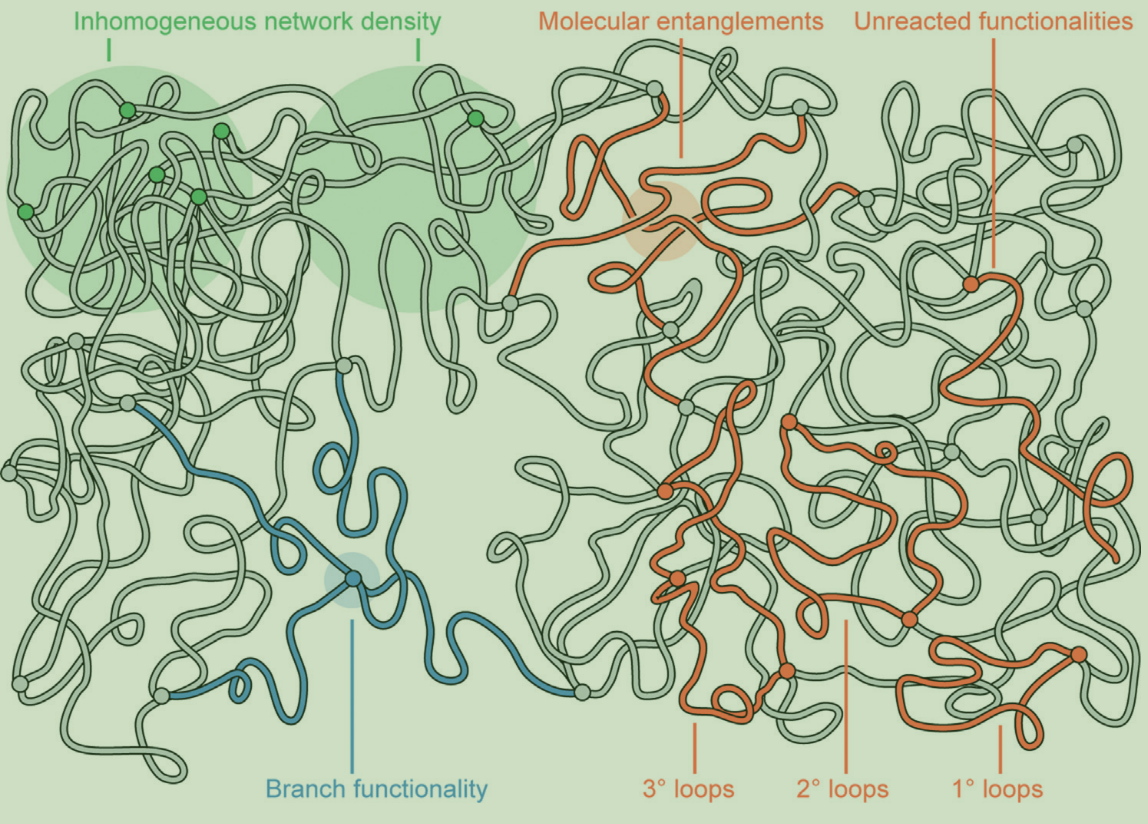
\includegraphics[width=0.8\textwidth]{figs/multilengthTopology.png}
    \caption{Multilength stuff. Scale from 10 to 100 nm shown in green, 1 to 10 nm shown in red and <1 nm shown in blue. }\label{fig:lengthScales}
\end{figure}

\subsection{Basic properties of Polymer Networks} 

\paragraph{Elasticity} The physical explanation of rubber elasticity comes from the reduction in conformational entropy that occurs as a strand in a network is stretched, this process is often modeled as the unwinding of flexible, random coils. 
Once the external stretching force is removed, an elastic entropic force restores the strands to their unstretched and higher entropy state. 
Therefore, it is concluded that network strands act as entropic molecular springs\citep{guPolymerNetworksPlastics2020}. 

\paragraph{Swelling} Polymer networks constructed from strong (e.g., covalent) bonds typically do not dissolve in solvents. 
Instead, such networks absorb solvent up to an equilibrium concentration and undergo a concomitant increase in volume. 
The equilibrium degree of swelling is dictated by a balance between the free energy of polymer-solvent mixing and the free energy cost of expanding the network, which is expressed by the Flory–Rehner equation[11,133]\footnote{for isotropic swelling of an affine polymer network [Eq. (12)]:
    \begin{gather*}
        \ln(1-\phi_{\mathrm{eq}}) + \phi_{\mathrm{eq}} + \xi\phi^2_{eq} = \eta_{eff}V_1(\phi_{\mathrm{eq}}/2-\phi^{1/3}_{eq})
    \end{gather*}
}

\paragraph{Viscoelasticity} Polymeric materials exhibit both viscous and elastic characteristics upon deformation, meaning that their properties may vary with the time scale or frequency at which measurements are performed. 
To characterize this viscoelasticity with respect to tensile, compressive, or shear deformation, several types of experimental measurements are commonly applied, such as stress relaxation, creep, and oscillatory shear tests\citep{guPolymerNetworksPlastics2020}. 

\newpage
